\section{Physics motivation\label{sec:physHI}}
\label{sec:physics}

In this Section we discuss the physics performance of the upgraded L1 trigger system for the 2018 high luminosity Pb-Pb run using three examples of measurements with rare probes. The performance of the upgraded system, which uses background subtraction for L1 event rejection and provides access to the full expected luminosity of 3~nb$^{-1}$ is compared to that of the current system. 
These examples illustrate the large improvements in statistical precision afforded by the improved ability to select jet events and high \pt\ particles with stage-2 L1 trigger upgrade during high luminosity Pb-Pb collisions. 

Below we discuss a selection of measurements which exploit the future high-luminosity data sets to 
provide important insights into the parton energy loss mechanism and heavy flavor particle production:

\begin{enumerate}
\item The flavor dependence of jet quenching is an important test ground for various parton energy loss models. 
Compared to light quarks, heavy quarks are expected to suffer from smaller radiative energy loss when passing through the medium because gluon radiation is suppressed at angles smaller than the ratio of the quark mass $M$ to its energy $E$~\cite{Dokshitzer:2001zm}. This effect (and its disappearance at high \pt) can be studied using charged particles, heavy flavor mesons and b-jets.
%\item Compared to quarks, gluons are expected to suffer a larger 
%energy loss because of the larger color factors. This effect can be studied using three-jet events.
\item Measurements of the charged particle and heavy flavor meson azimuthal anisotropy ($v_2$) at very high \pt\ give access to the in-medium path-length 
dependence of energy loss. The azimuthal anisotropy as a function of particle \pt\ also yields important information about the parton energy dependence of the energy loss.  At the low \pt, hadronization of heavy quarks such as parton-to-jet fragmentation and the recombination of heavy quarks and light flavors has a significant impact on the magnitude of the heavy flavor meson $v_2$. 
\item Studies of jet-heavy flavor meson correlation could give important insights into the parton energy loss mechanism and for the studies of medium induced radiation and medium response to the energetic heavy quarks.
\end{enumerate}

These and other measurements rely on a sufficiently selective jet and heavy flavor meson trigger to provide access to the full delivered luminosity. At the same time, a large minimum-bias sample is needed in order to access to very low \pt\ heavy flavor mesons and to perform data-driven tracking and jet energy corrections.  To illustrate the impact of the L1 rate upgrade, data collected during the 2015 Pb-Pb run were used to estimate physics reach for a future high-luminosity run (assuming $L_{int} =$3~nb$^{-1}$) for these three physics cases. 


\subsection{Nuclear Modification Factors of Heavy Flavor Mesons}

One of the proposed observables that reveal the flavor dependence of in-medium parton energy loss is the reduction of heavy flavor meson yield. This can be studied by measurements of nuclear modification factors ($R_{AA}$), defined as the ratio of the yield in nucleus-nucleus collisions to that observed in pp collisions, scaled by the number of binary nucleon-nucleon collisions. Theoretical calculations of $R_{AA}$ for fully reconstructed D and B mesons are shown in Figure~\ref{fig:RAA_theory}. At low \pt, the production rate of heavy flavor meson in Pb-Pb is sensitive to the elastic energy loss of the heavy quark, gluon shadowing effect in the nuclear parton distribution function. and the rate of recombination of the heavy quark and light flavors at the hadronization stage. At high \pt, the size of the suppression is sensitive to the heavy quark radiative energy loss in the pQCD based models. Precision measurement of the $R_{AA}$ from intermediate \pt ($\sim 10$ GeV) to very high \pt (200-400 GeV) could the pathlength dependence of the heavy quark energy loss and potentially to distinguish models based on AdS/CFT and pQCD. 

\begin{figure}[!ht]
\begin{center}
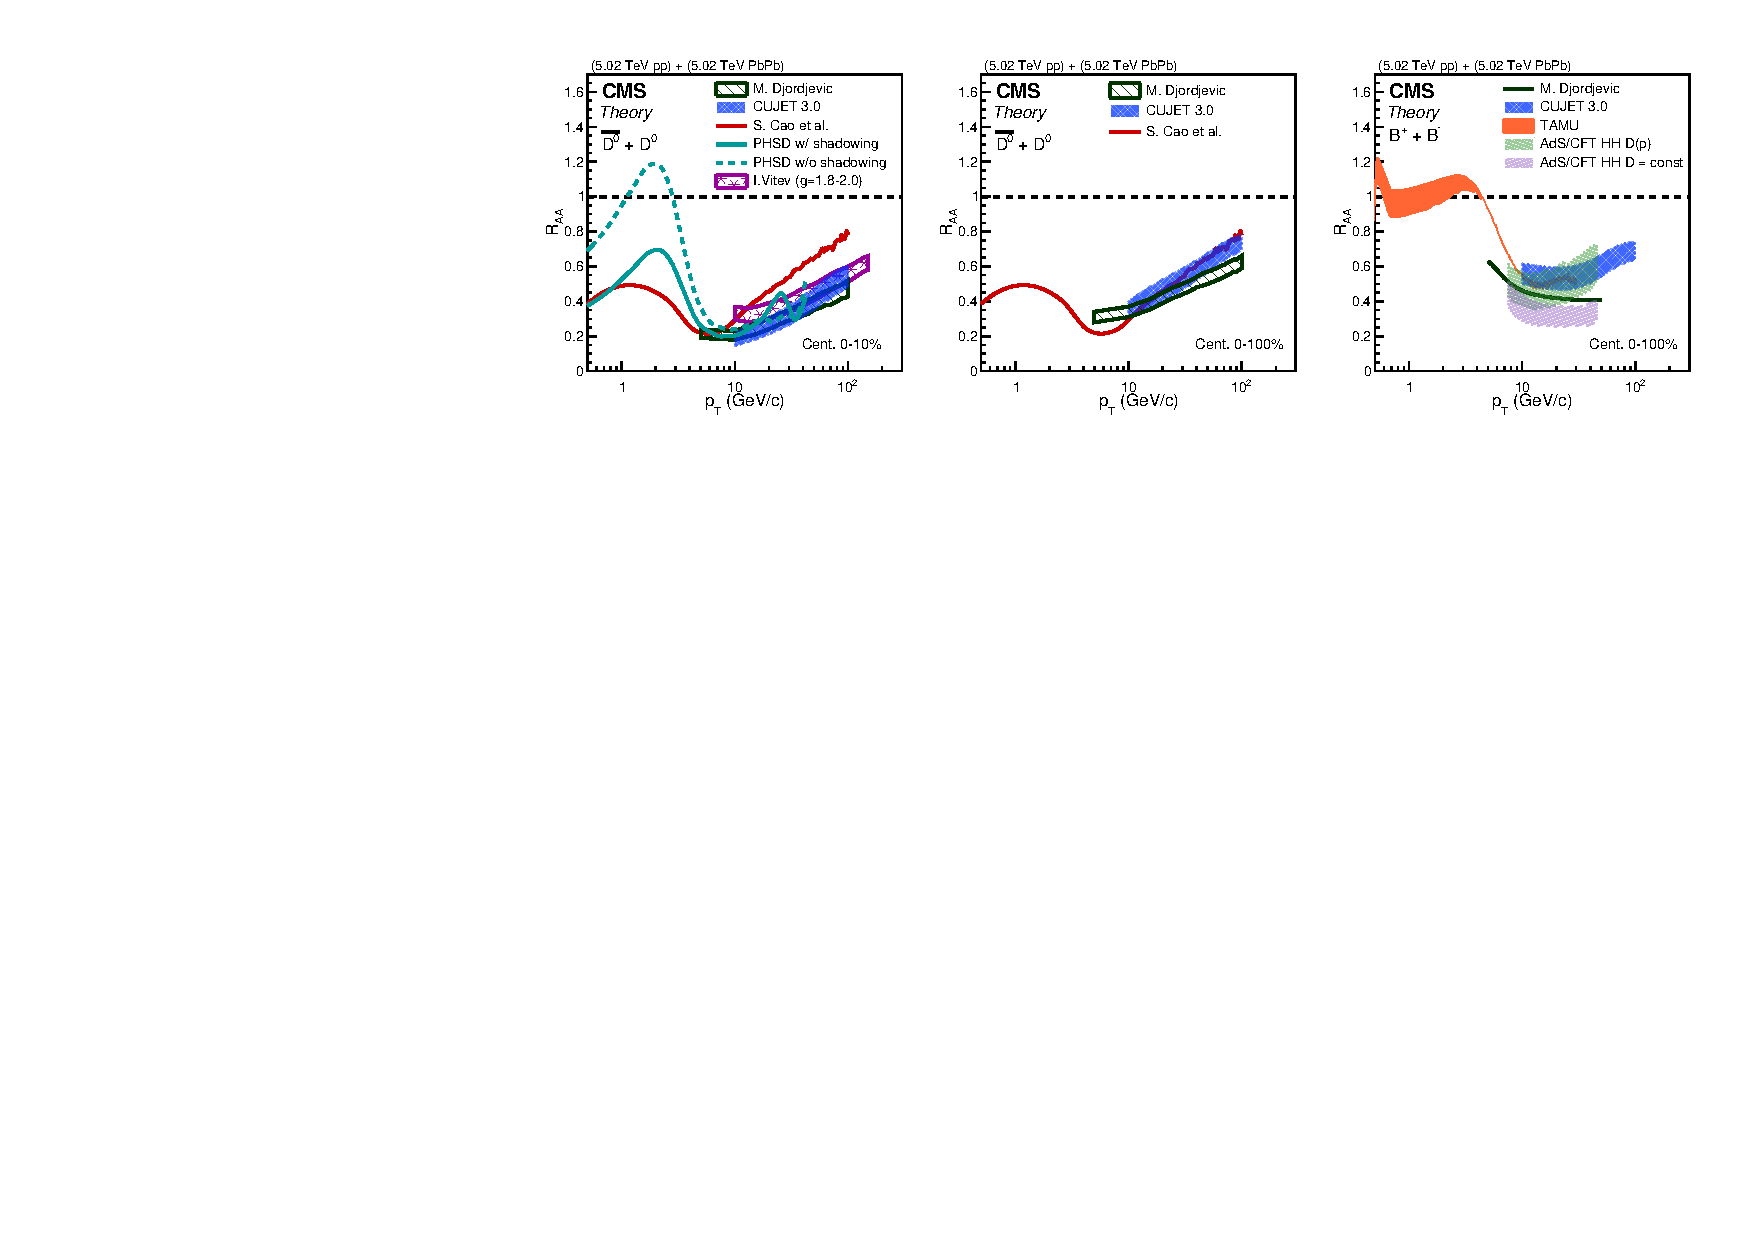
\includegraphics[width=.98\textwidth]{figures/cTheoryRAA_BD_v1.pdf}
\caption{Theoretical calculations of nuclear modification factors of charged particles, $D^0$ and $B^+$ mesons.}
\label{fig:RAA_theory}
\end{center}
\end{figure}

It is also predicted that a significant fraction of the low \pt\ heavy quarks could hadronize via recombination with other quarks from the medium. These motive measurements of the $R_{AA}$ from $D^0$, $D^+$, ($B^+$), $D_s^+$ ($B_s$) and $\Lambda_c$ ($\Lambda_b$) which could provide crucial information about the interactions of the heavy quarks and the produced medium. Especially, the $D_s$ and $B_s$ measurements are sensitive to the strangeness content of the produced strongly interacting medium. Figure~\ref{fig:HFMesonMass} shows the performance of $D^+\rightarrow \phi\pi^+$, $D_s^+\rightarrow \phi \pi^+$, $\Lambda_c\rightarrow p K^-\pi^+$ and $B^+\rightarrow \bar{D}^0 \pi^+$ reconstruction in the heavy ion collisions with the CMS detector, projected to the expected statistics to be collected with the L1 trigger rate upgrade. Significant signals of $D_s^+$ and $\Lambda_c$ could be observed which enable the measurement of Ds and $\Lambda_c$ $R_{AA}$ for the first time. 


\begin{figure}[!ht]
\begin{center}
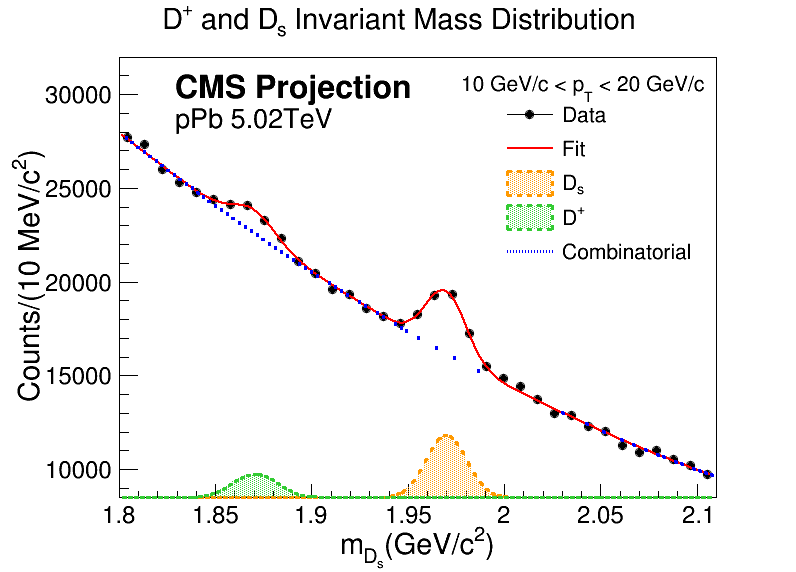
\includegraphics[width=.32\textwidth]{InvMassFigures/Ds.png}
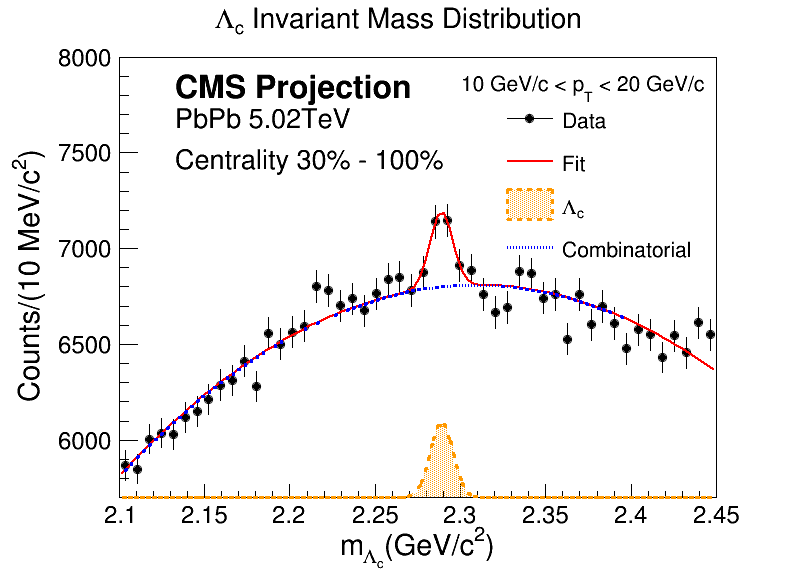
\includegraphics[width=.32\textwidth]{InvMassFigures/LambdaC.png}
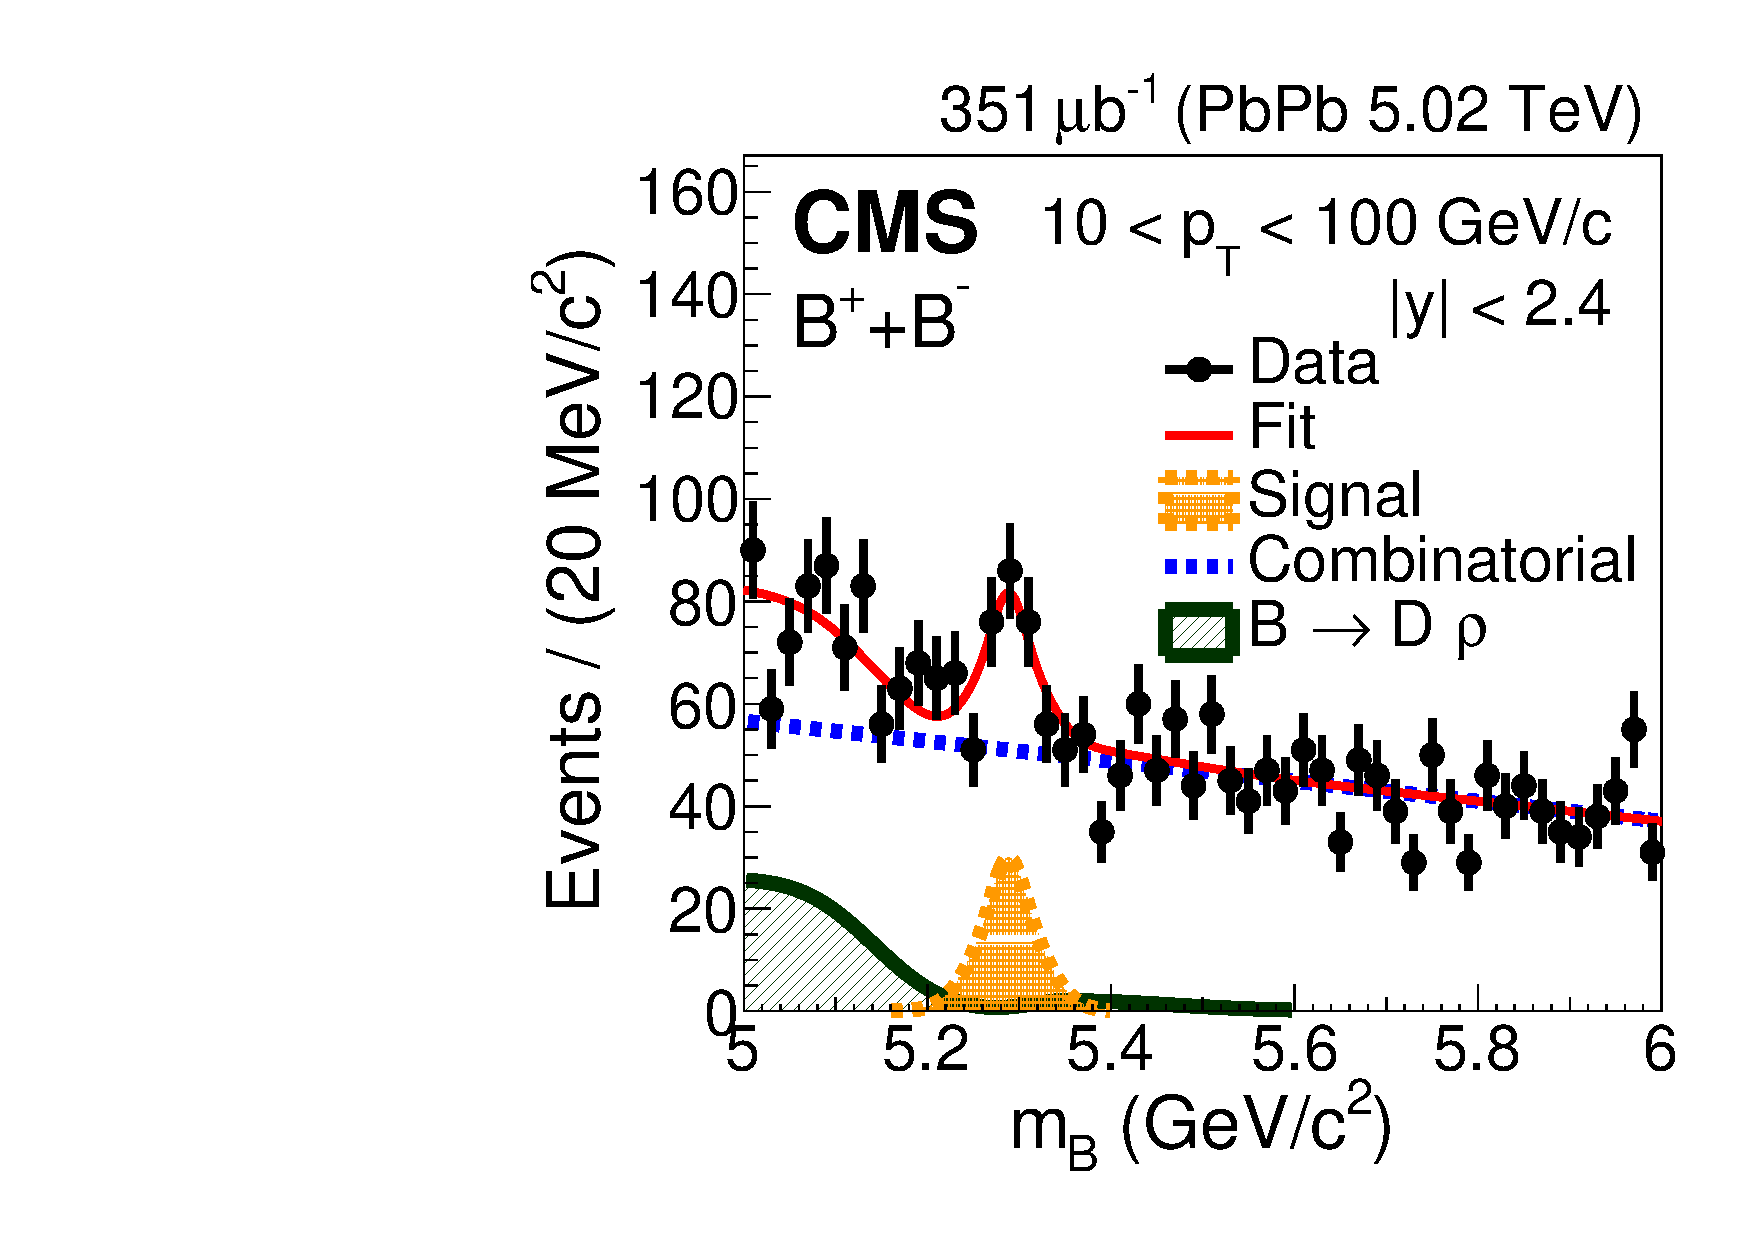
\includegraphics[width=.335\textwidth]{InvMassFigures/BtoDpi_data_PbPb_10_100.pdf}
\caption{Invariant mass distributions}
\label{fig:HFMesonMass}
\end{center}
\end{figure}

Figure~\ref{fig:RAA_2015} shows the expected performance with the data recorded in 2015 and the projected performance in 2018 and beyond. With the high statistics jet and heavy flavor triggered sample, the precision of the $R_{AA}$ measurements at high \pt could be greatly improved by jet and heavy flavor triggered sample. At the same time, with the L1 trigger rate upgrade proposed in this proposal, the much larger minimum-bias sample enables CMS to perform these studies down to the very low \pt region. The expected precision of $D^0$, $B^+$ and $D_s$ $R_{AA}$ measurements from low \pt to high \pt could provide a strong constraint on the theoretical models and the difference in the suppression magnitude between those mesons could be observed for the first time.


\begin{figure}[!ht]
\begin{center}
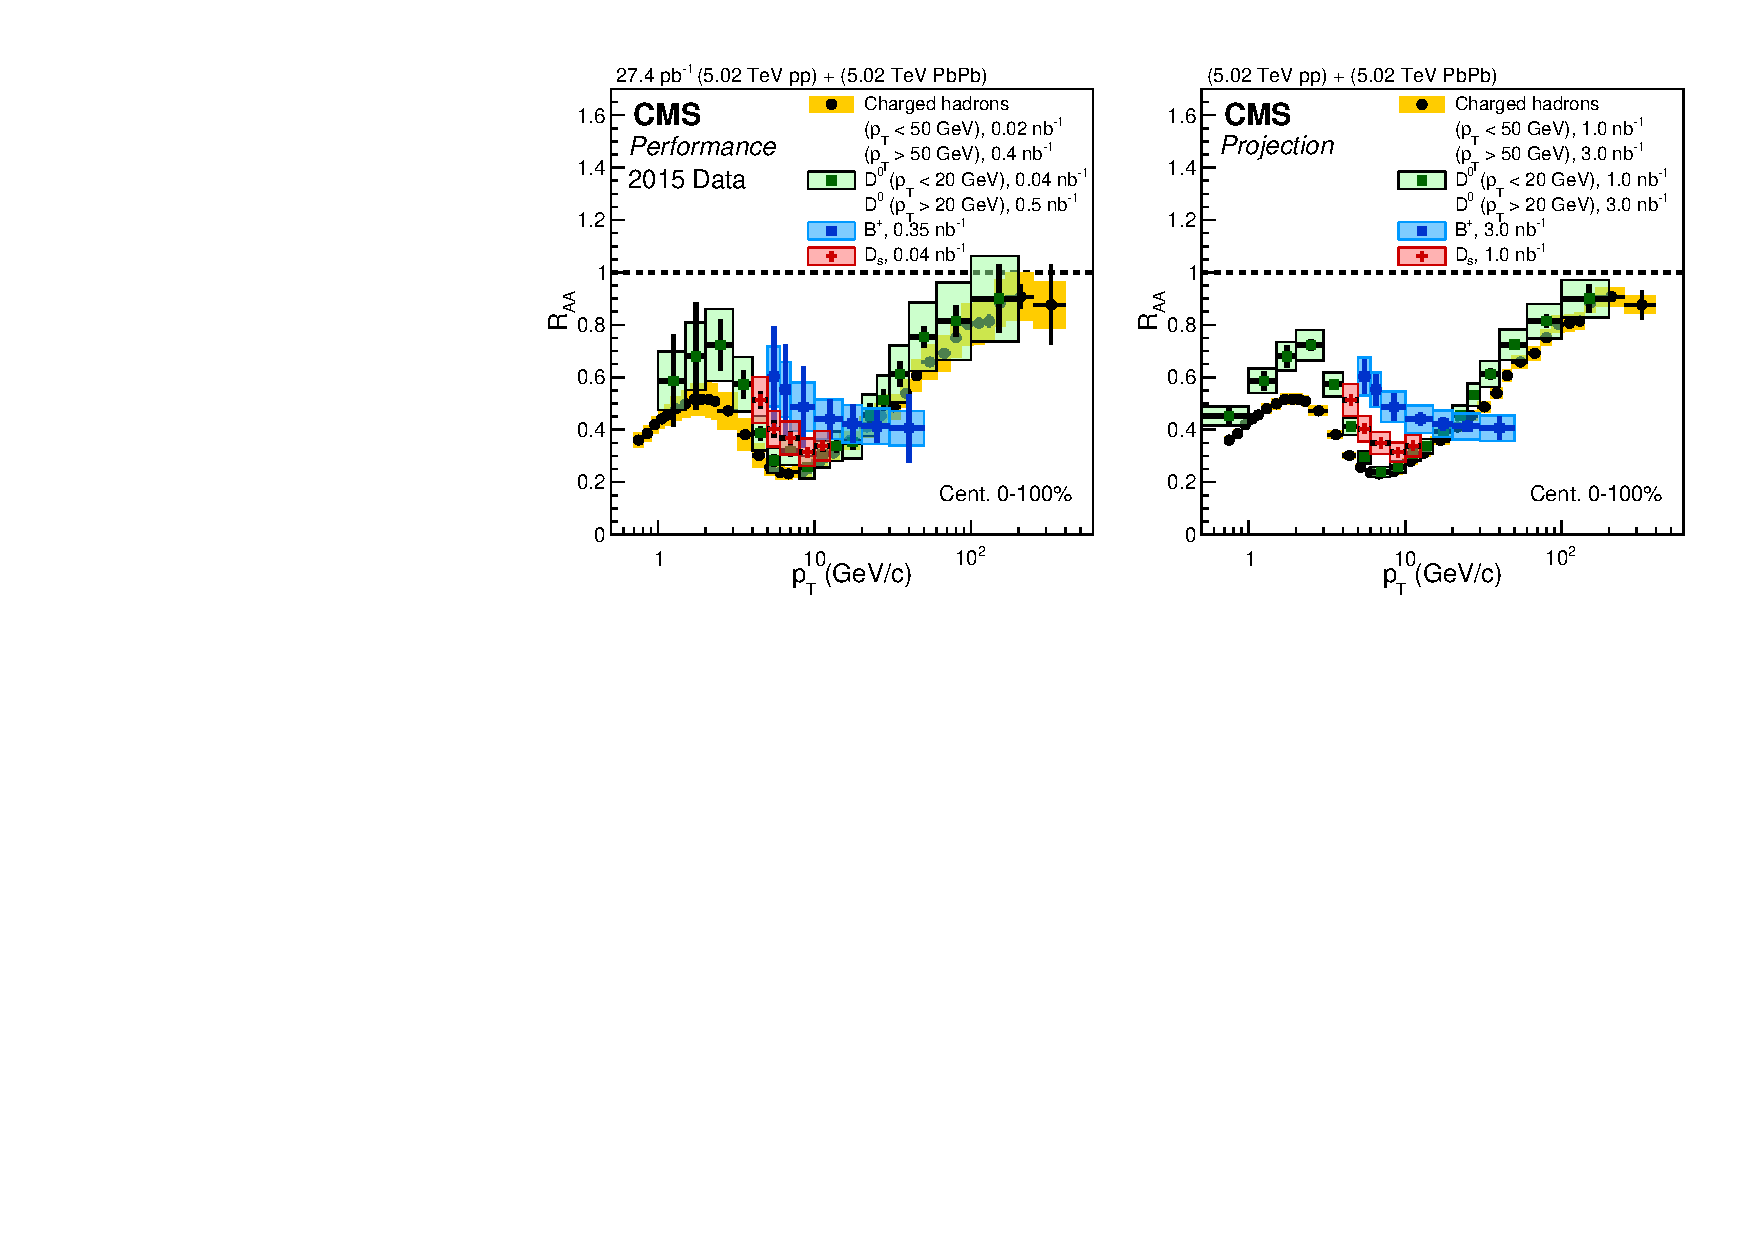
\includegraphics[width=.98\textwidth]{figures/cRAA_lumiTG_3_lumiMB_1_v2.pdf}
\caption{Nuclear modification factors of charged particles, $D^0$, $D_s$ and $B^+$ mesons with 2015 data (left panel) and the statistics expected with L1 trigger rate upgrade.}
\label{fig:RAA_2015}
\end{center}
\end{figure}

\subsection{Azimuthal anisotropy of Heavy Flavor Mesons}

Azimuthal anisotropy of hadrons provides information about their production with respect to the reaction plane ($\Psi_n$). At high \pt, the larger in-medium path-length of the mother partons emitted in the direction of the reaction plane leads to a stronger suppression of the yield due to jet quenching. Therefore, measurements of the $v_n$ coefficients from Fourier expansion of the particle distributions $dN/d\psi$ are sensitive to path length dependence of the parton energy loss. At low \pt, a large $v_2$ (elliptic flow) signal is considered as an evidence for collective hydrodynamical expansion of the medium. Measurements of heavy flavor meson $v_n$ could provide important information about the thermalization of the heavy quarks in the medium. Precision measurements of the $v_n$ as a function of heavy flavor meson \pt could teach us how the azimuthal anisotropy of the light flavor partons contribute to the observed anisotropy through the recombination of heavy quarks and light quarks. As shown in Figure~\ref{v2_theory}, the predicted elliptic flow ($v_2$) signal covers a large range of values due to the difference in the treatments of in-medium parton transport and parton energy loss. Figure~\ref{fig:v2_projection} shows the expected performance of elliptic flow ($v_2$) measurements with the data recorded in 2015 and the projected performance in 2018 and beyond. The new precise data will be able to constrain various components of the theoretical models, to determine the heavy quark diffusion coefficient in QGP, and to reveal flavor dependence of the parton energy loss.


\begin{figure}[!ht]
\begin{center}
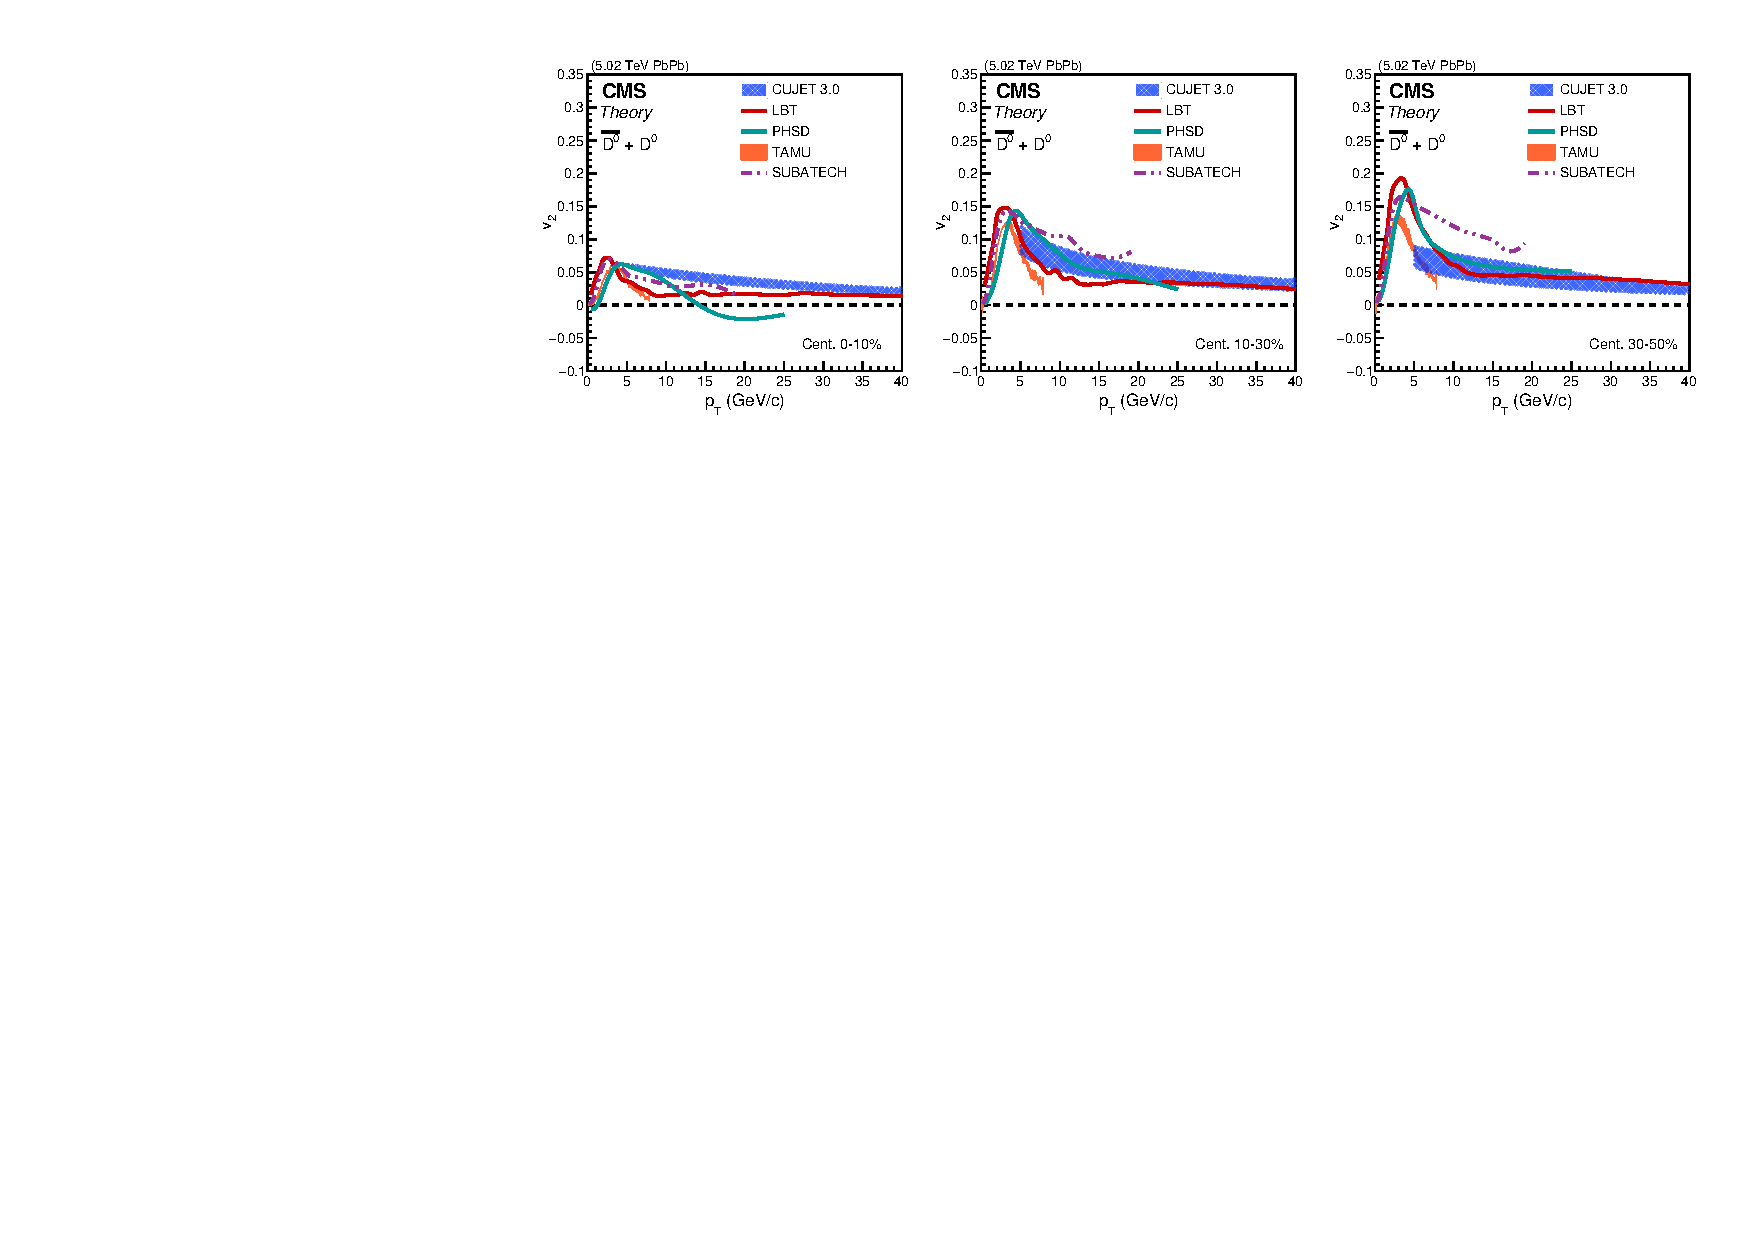
\includegraphics[width=.98\textwidth]{figures/cTheoryV2_D_v1.pdf}
\caption{Theoretical calculations of v2.}
\label{fig:v2_theory}
\end{center}
\end{figure}

\begin{figure}[!ht]
\begin{center}
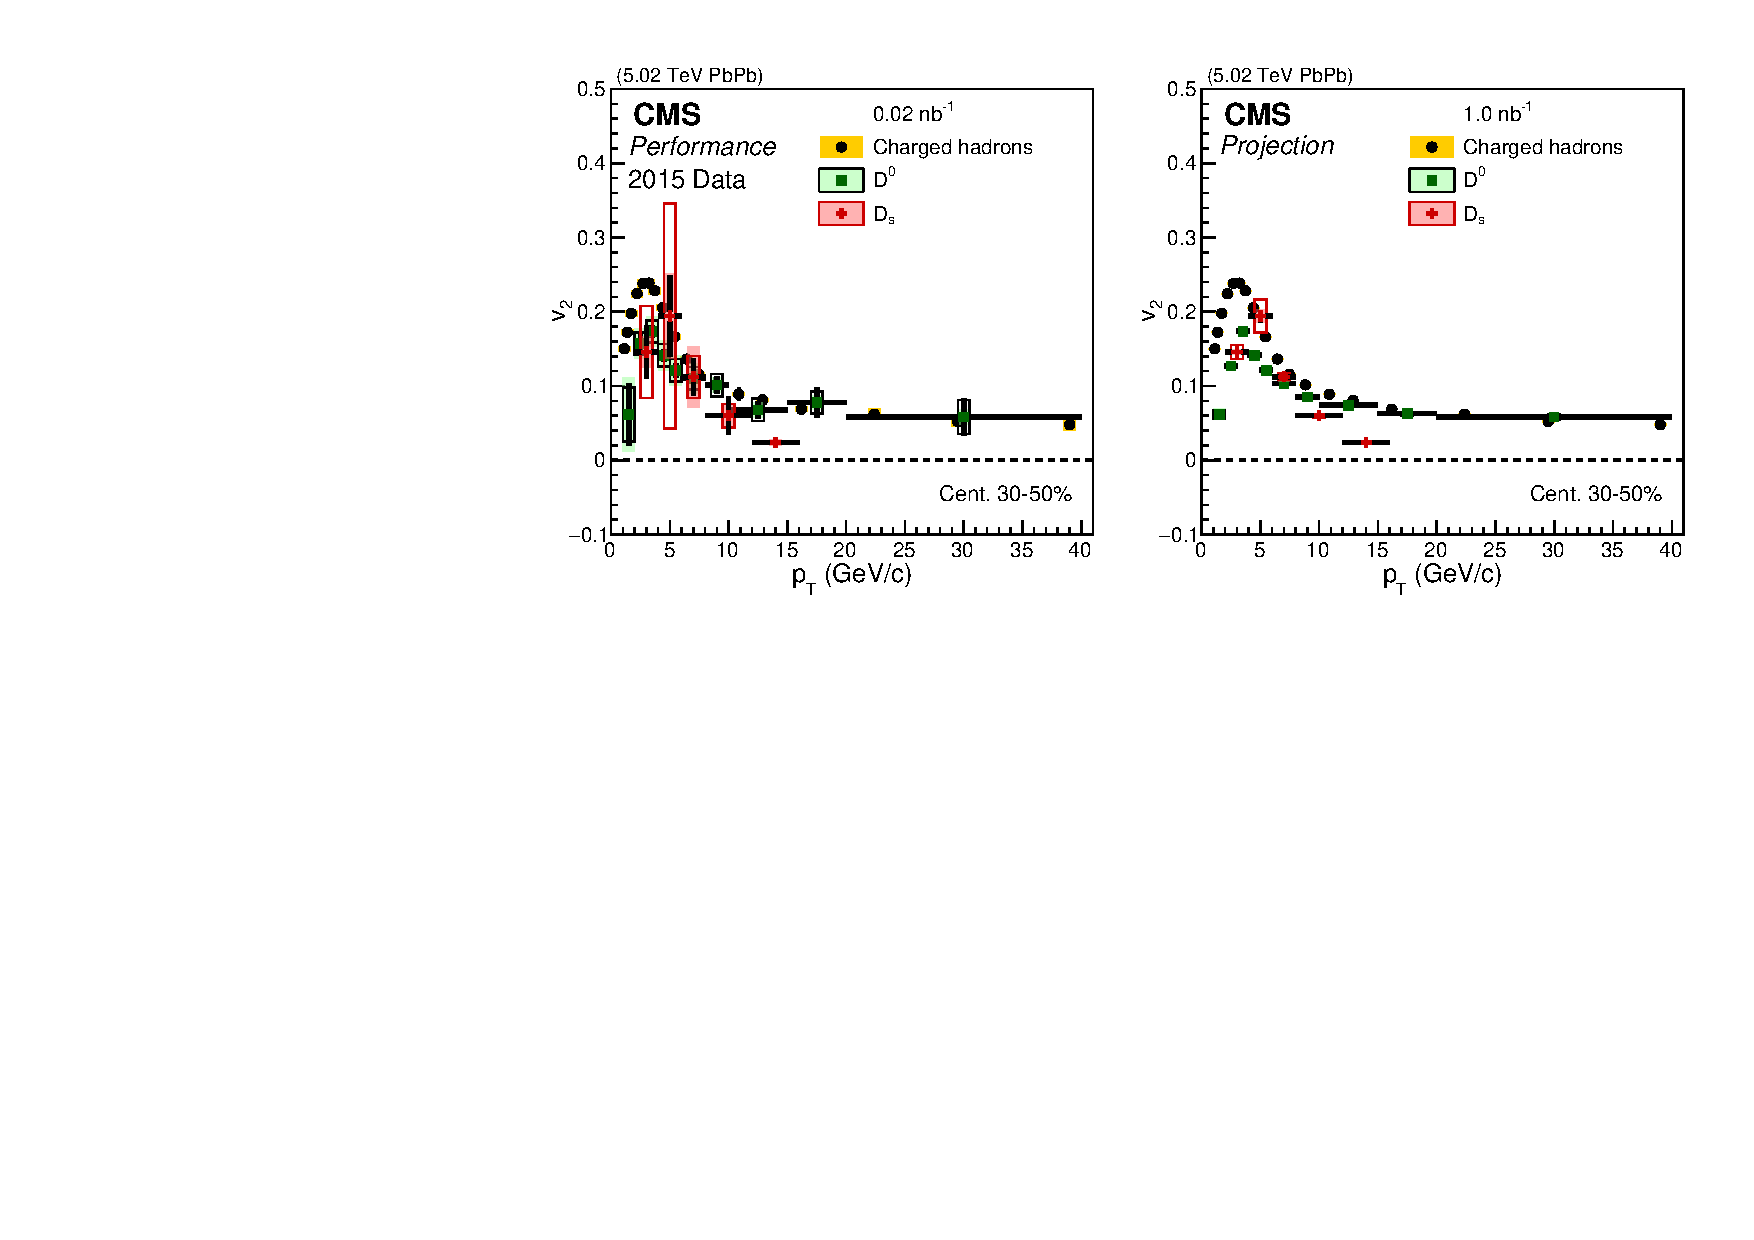
\includegraphics[width=.98\textwidth]{figures/cV2_lumiMB_1.pdf}
\caption{V2 measurement.}
\label{fig:v2_projection}
\end{center}
\end{figure}



\subsection{$D^0$-Jet and $D^0$-hadron correlations}
{\bf [To be updated]}

CMS has published jet-hadron and jet shape and dijet missing transverse momentum measurements which showed a significant modification of the angular structure of the jets. A significant amount of energy is transferred to very large angle with respect to the jet axis.
Studies of $D^0$-jet and $D^0$-hadron angular correlation are sensitive to energy loss mechanism. 

\begin{figure}[!ht]
\begin{center}
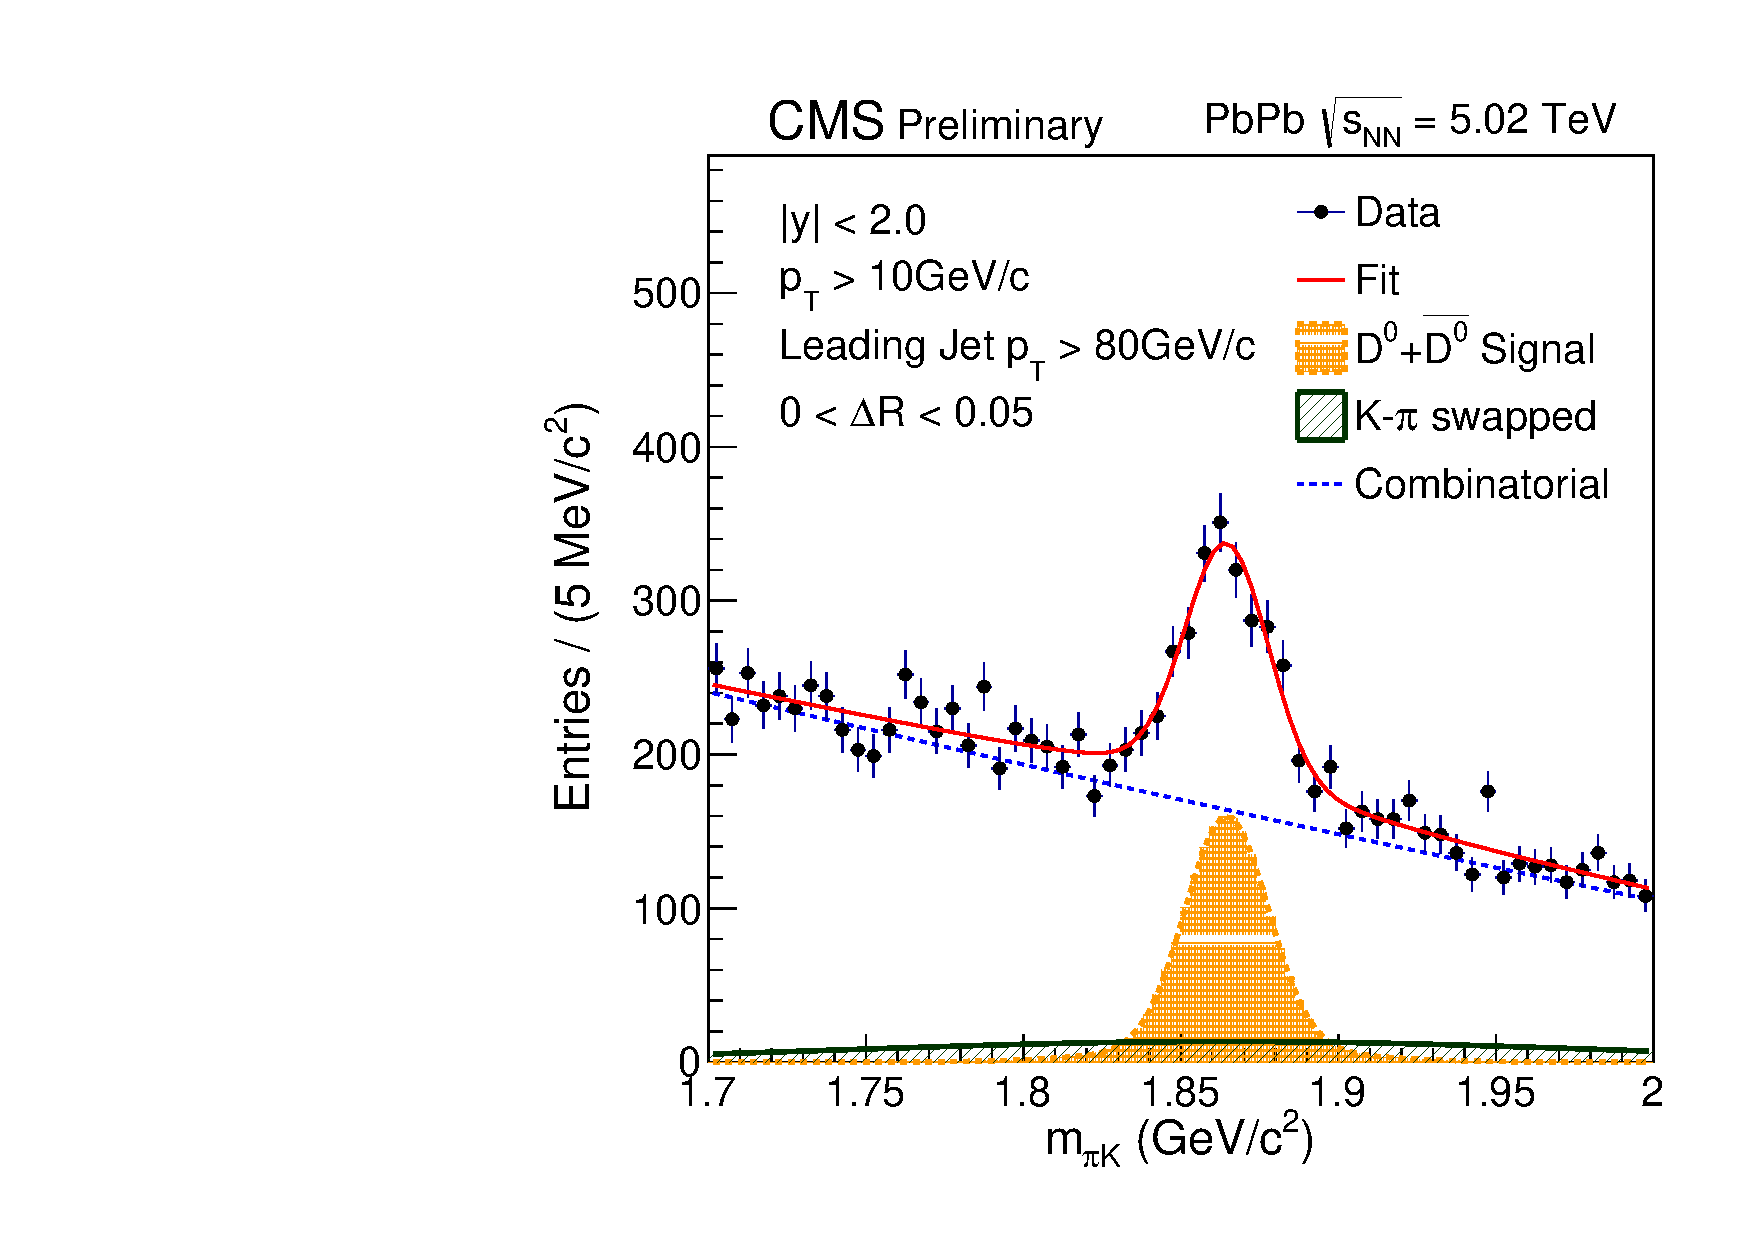
\includegraphics[width=.49\textwidth]{DJetPlots/fhHistoMass_R0.pdf}
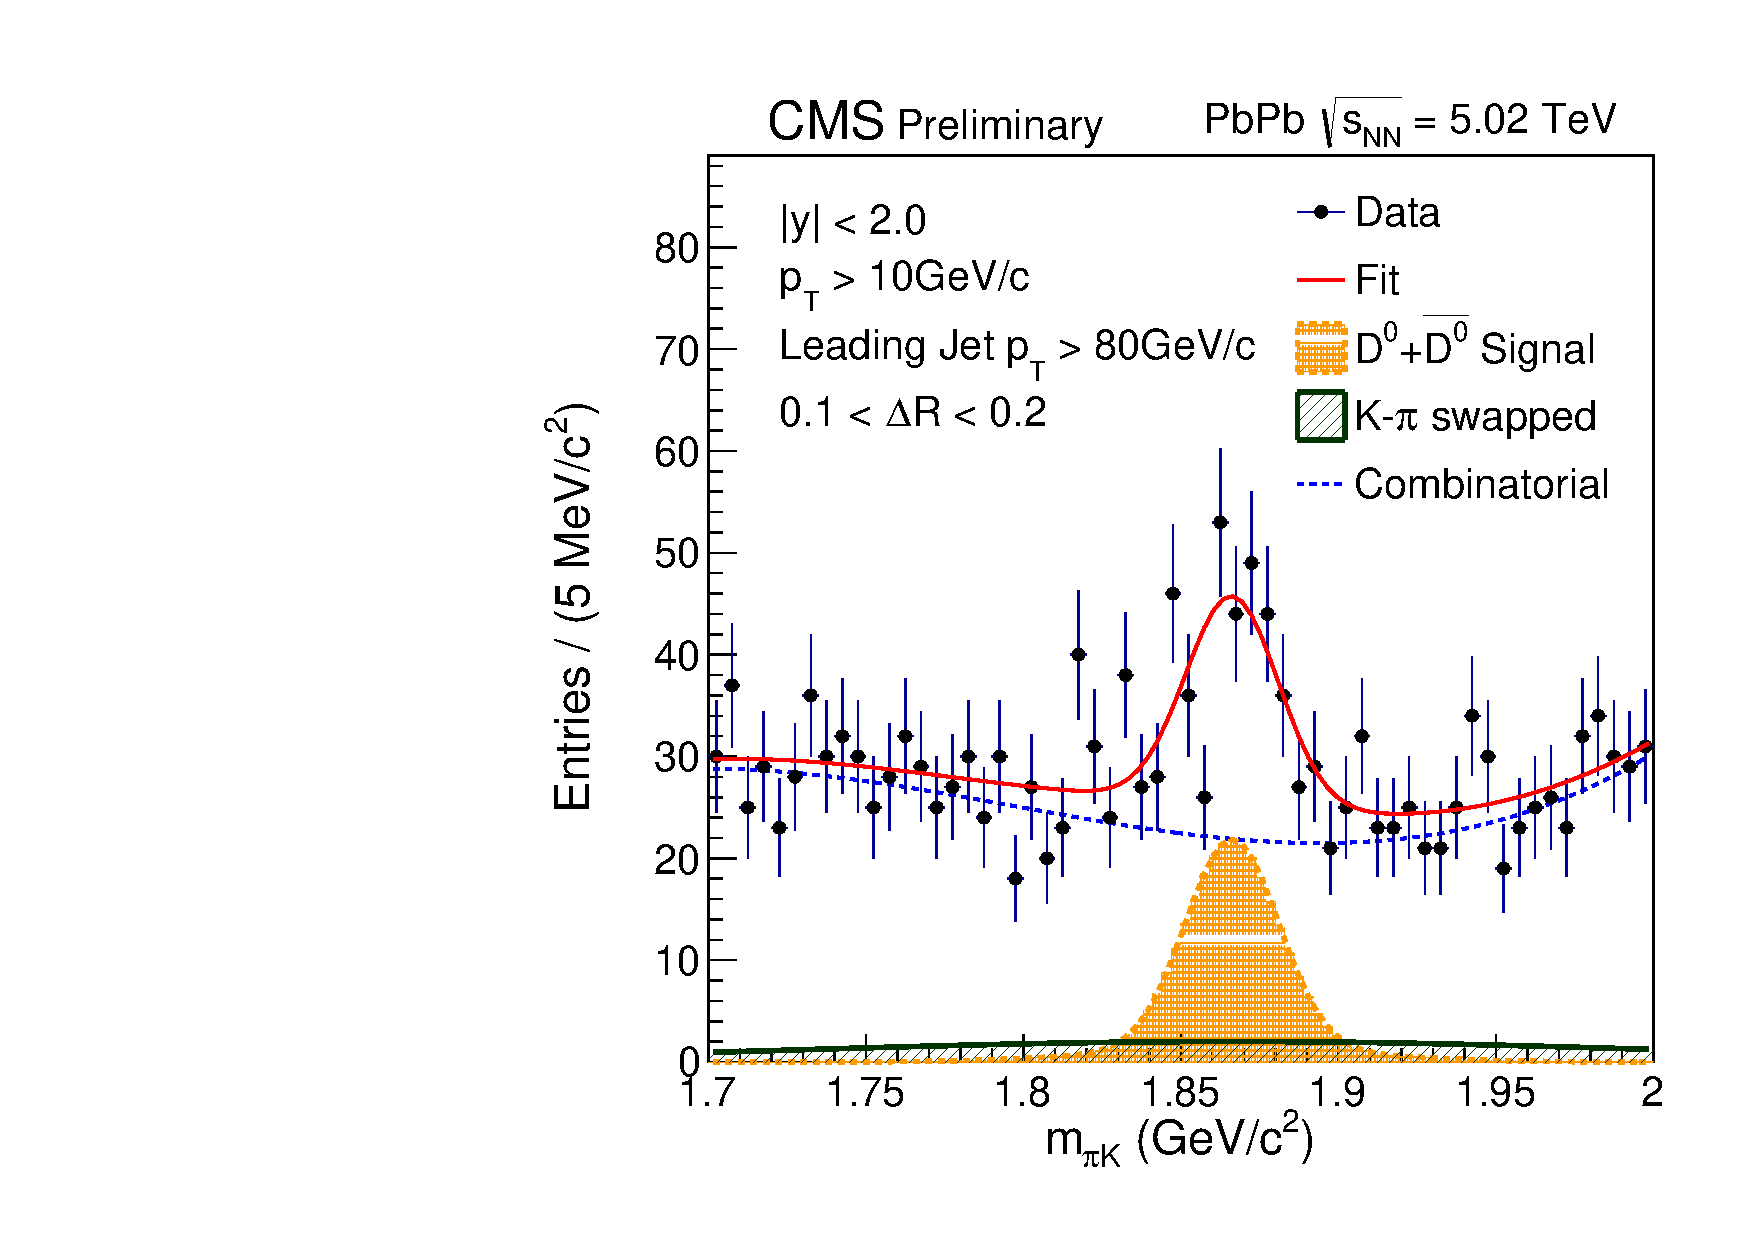
\includegraphics[width=.49\textwidth]{DJetPlots/fhHistoMass_R2.pdf}
%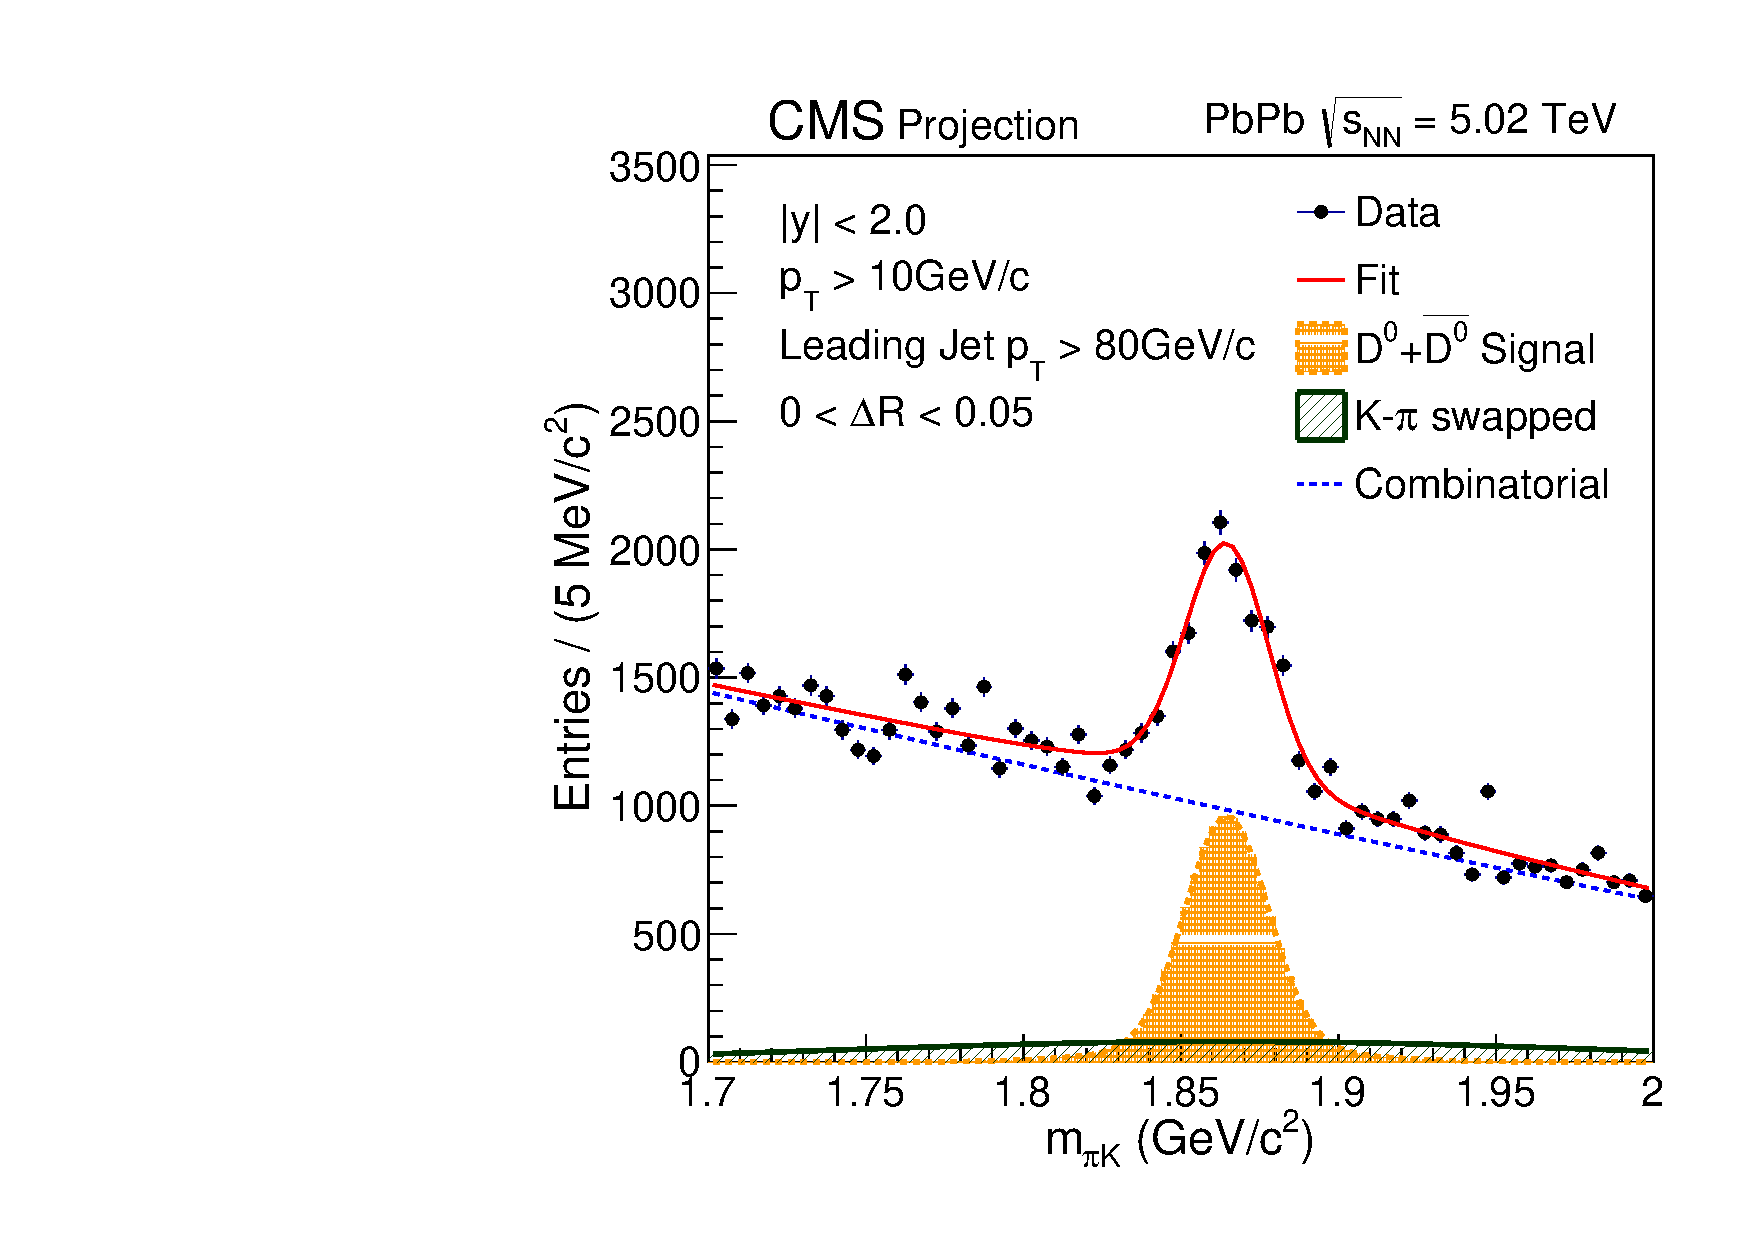
\includegraphics[width=.49\textwidth]{DJetPlots/fhHistoMass_R0Scaled.pdf}
%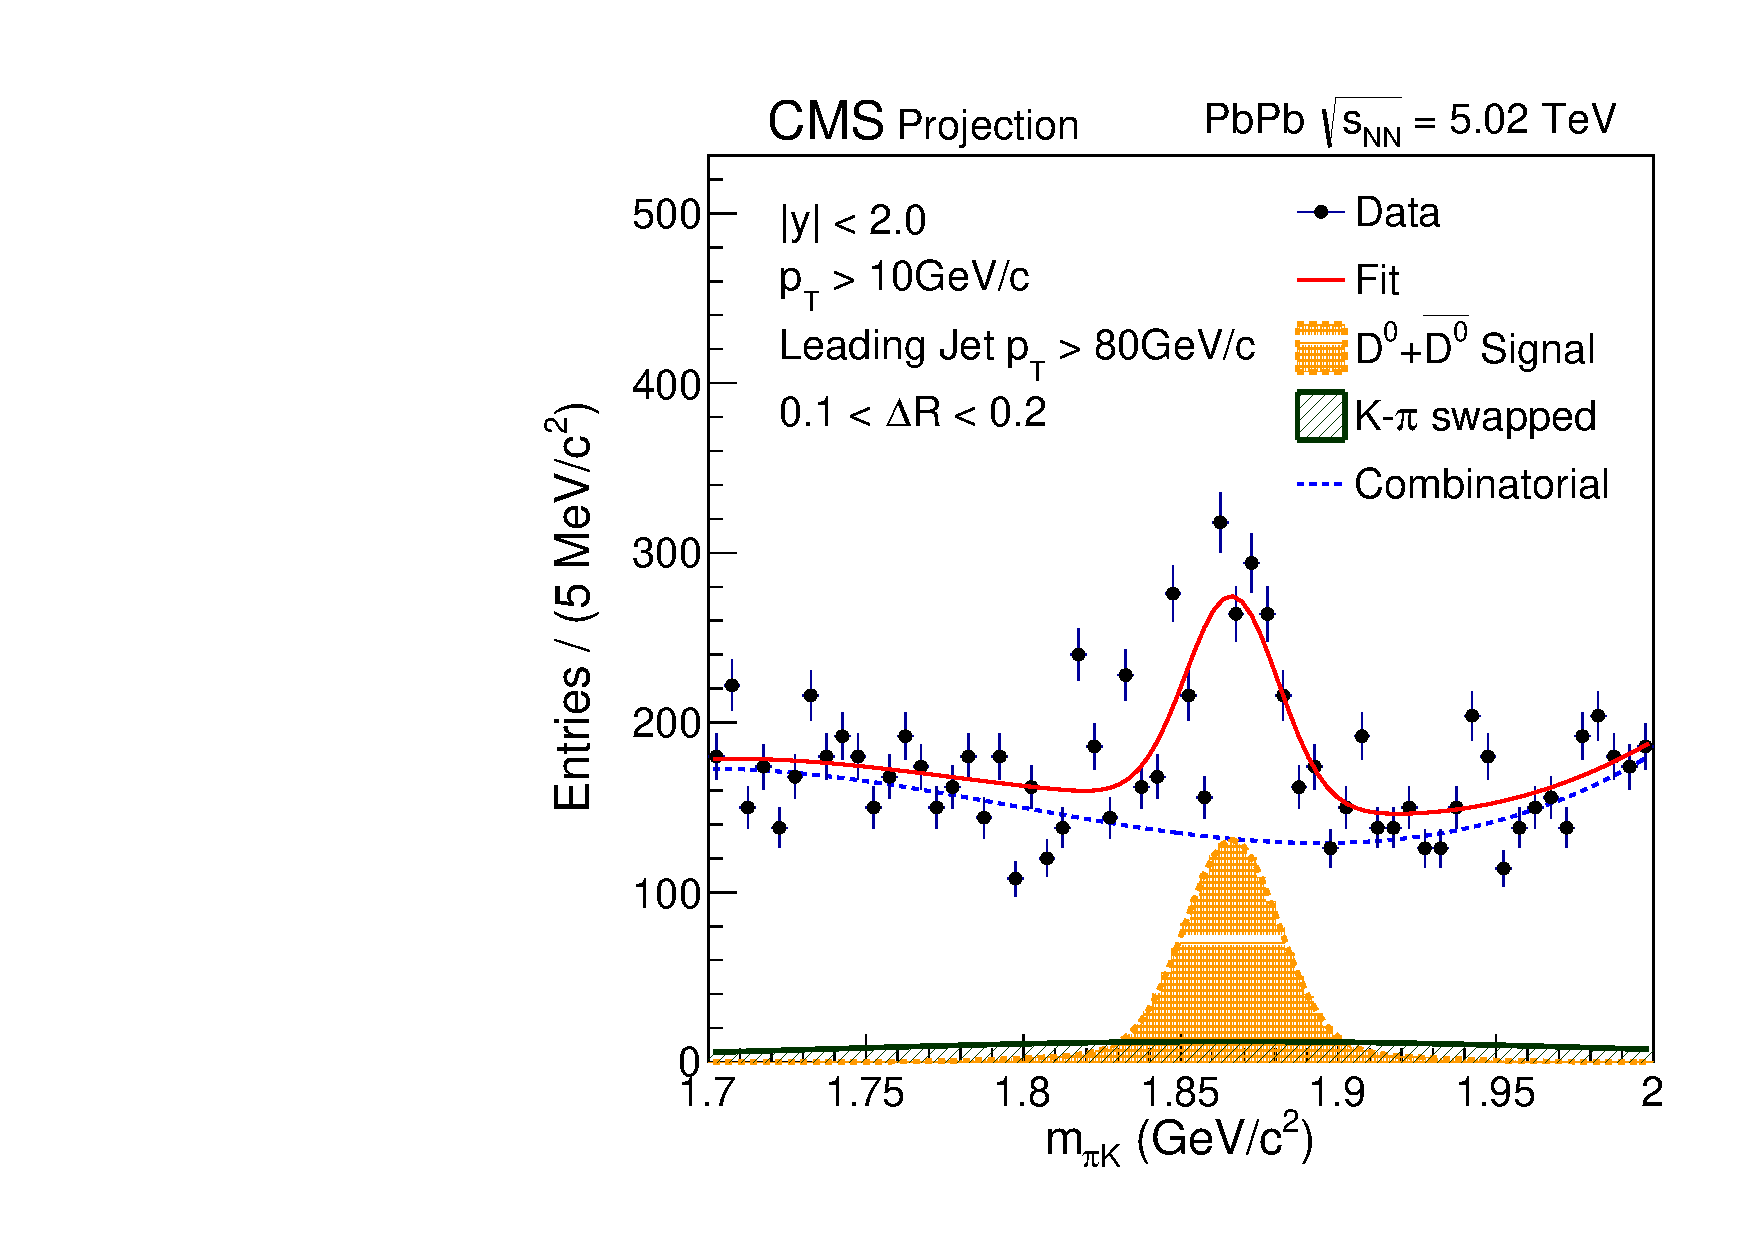
\includegraphics[width=.49\textwidth]{DJetPlots/fhHistoMass_R2Scaled.pdf}
\caption{}
\label{fig:D0_Jet}
\end{center}
\end{figure}

\begin{figure}[!ht]
\begin{center}
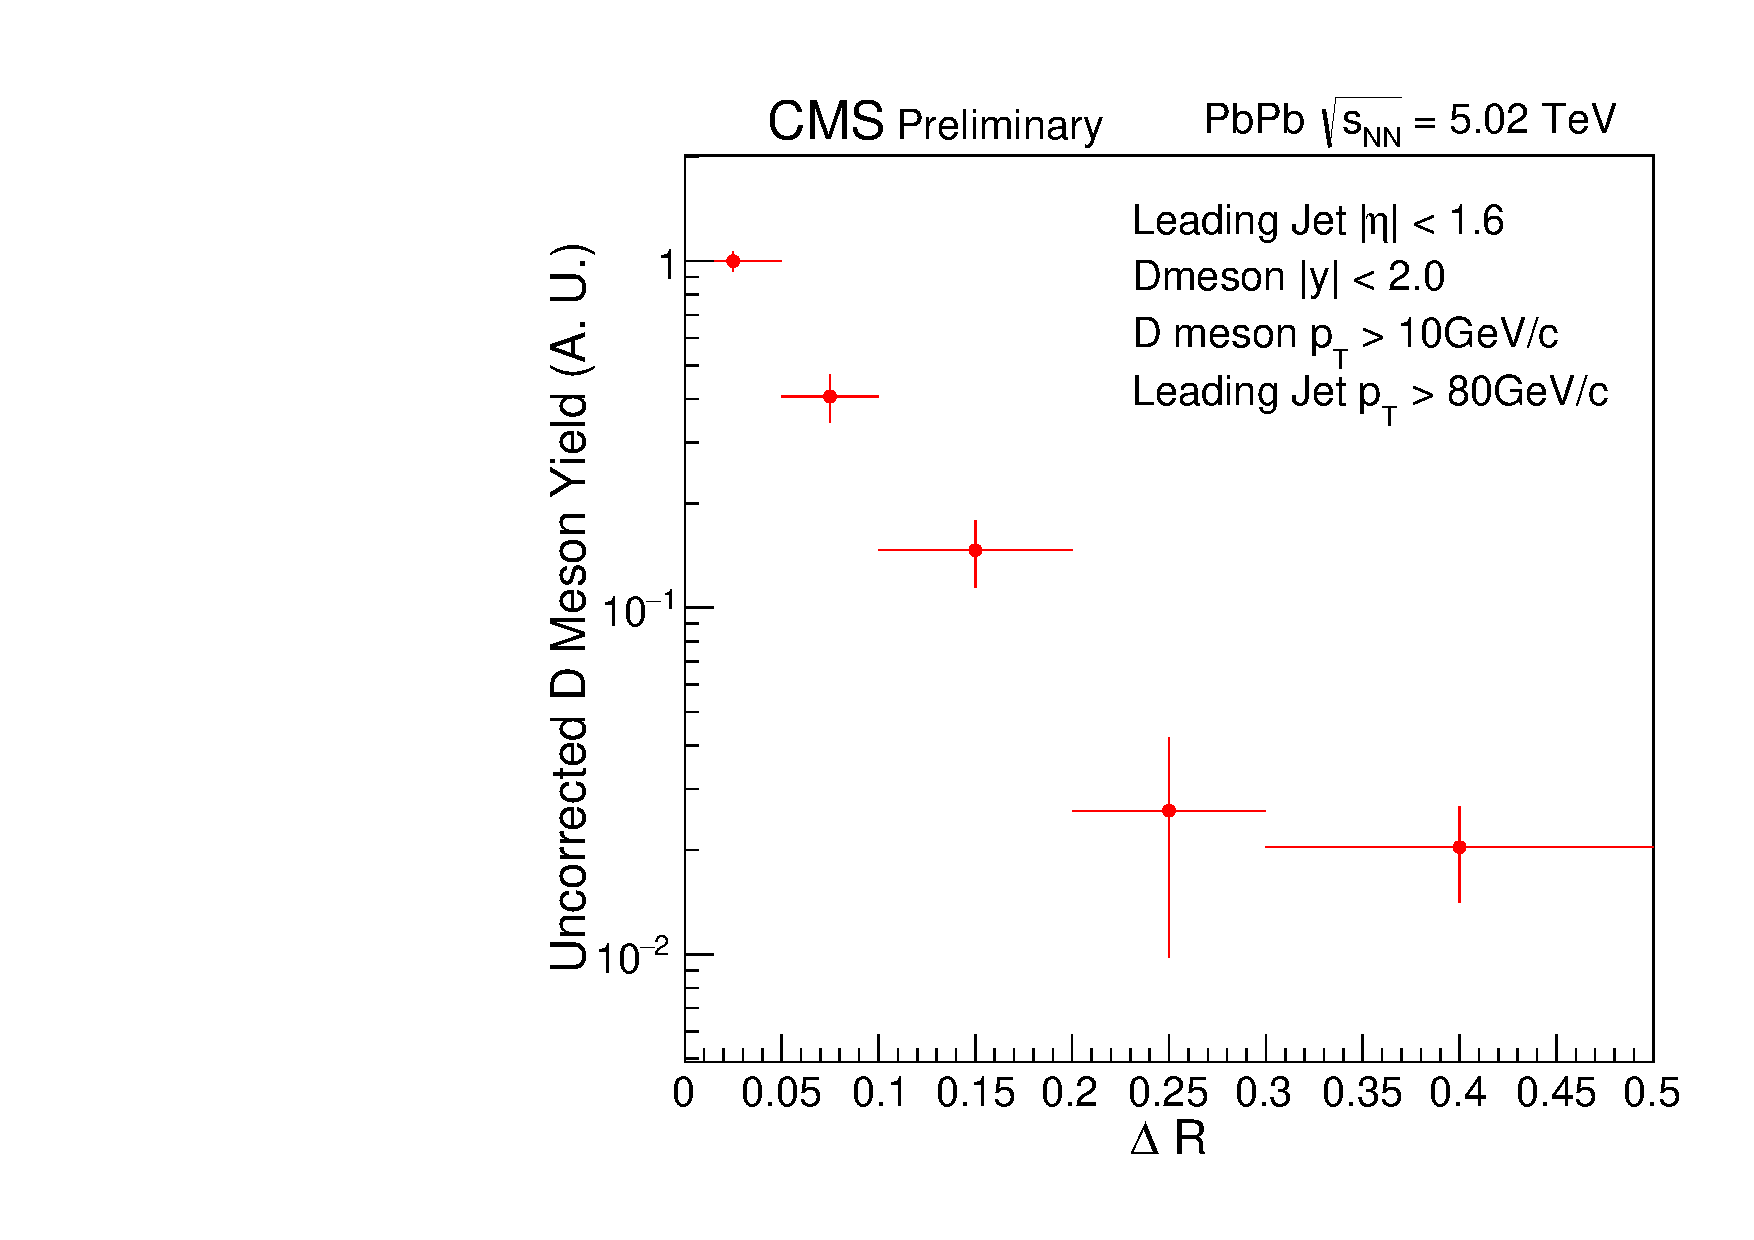
\includegraphics[width=.49\textwidth]{DJetPlots/PrelimYield.pdf}
%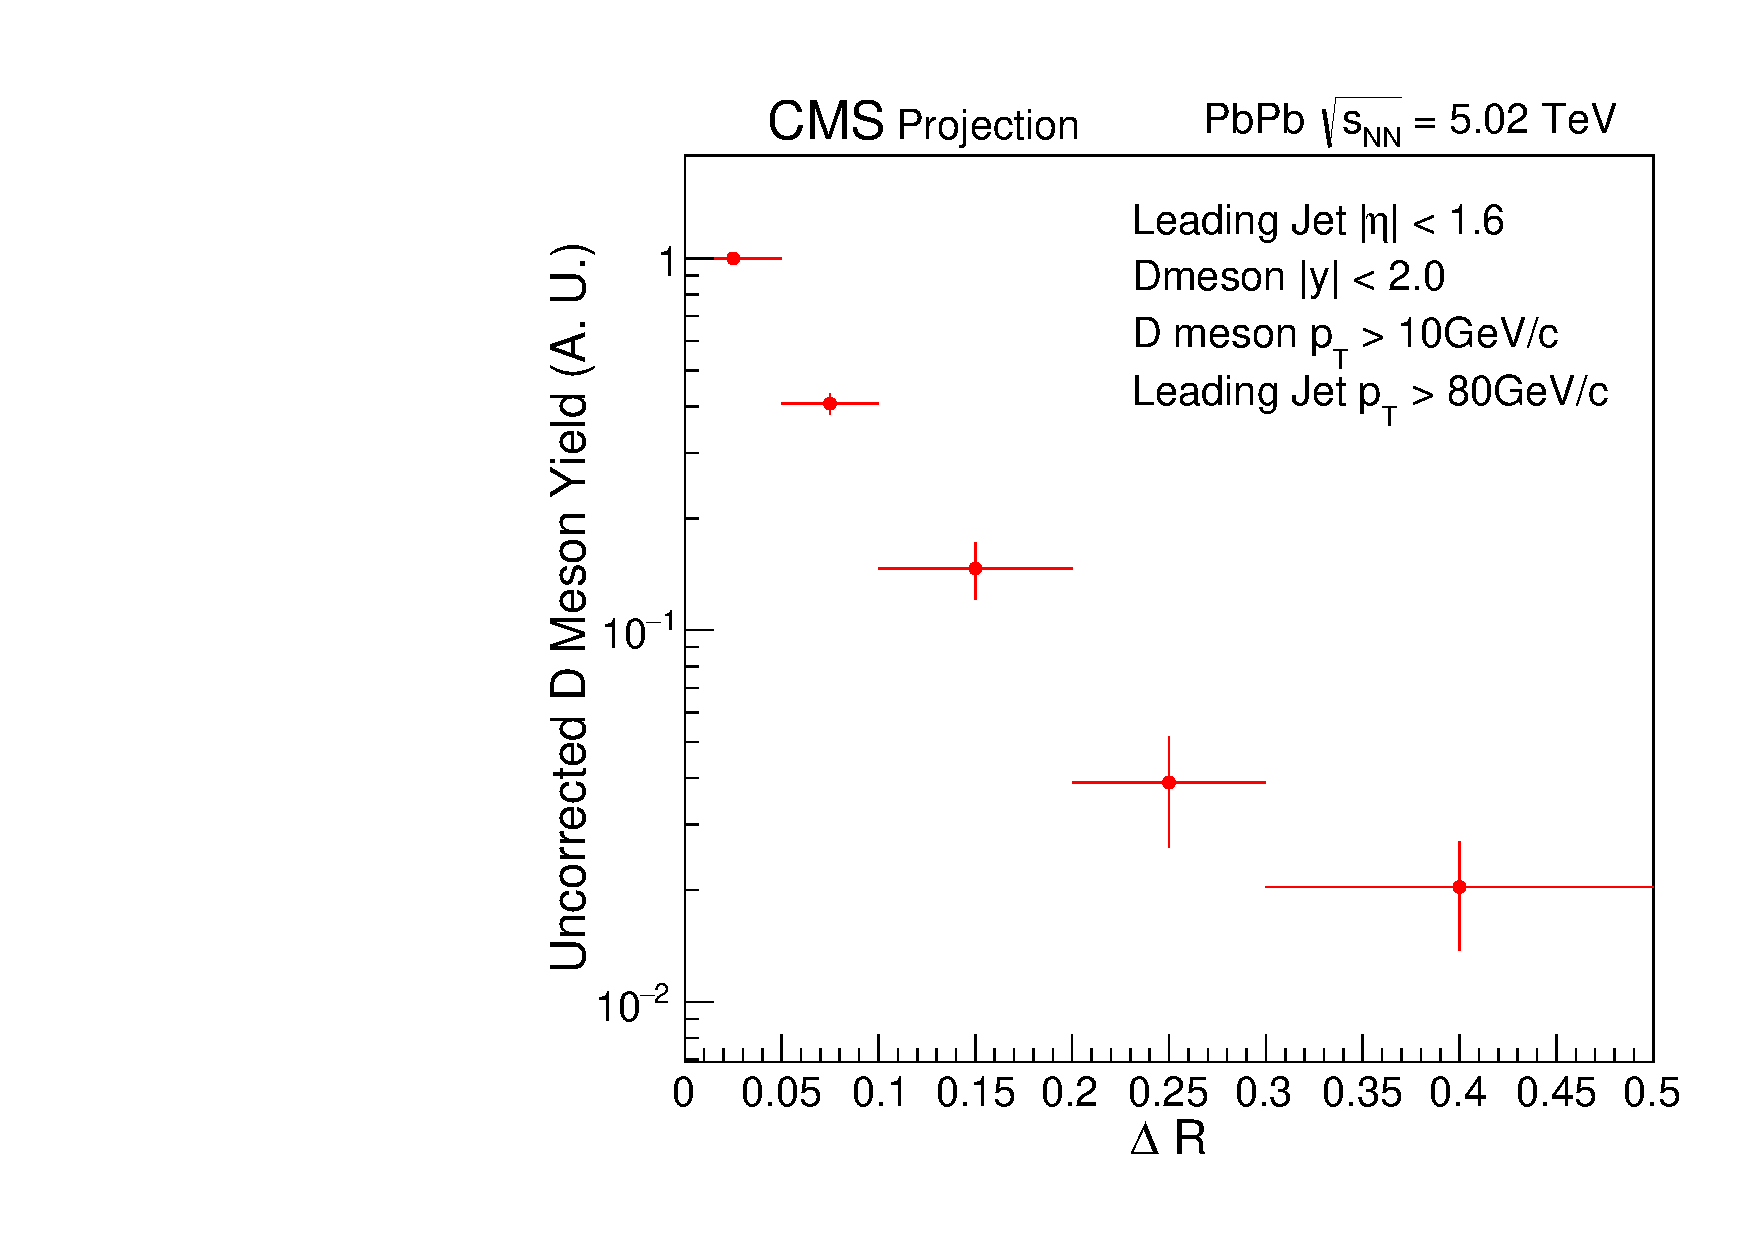
\includegraphics[width=.49\textwidth]{DJetPlots/ProjectionYield.pdf}
\caption{}
\label{fig:D0_JetYield}
\end{center}
\end{figure}


\subsection{Summary}

The current and projected physics performance of various measurements are shown in Table~\ref{physicsSummary}. With the proposed works on the stage-2 Level 1 trigger upgrade and detector readout, the kinematic range covered by CMS could be greatly increased and many more observables which are not yet accessible with 2015 data will become feasible for the first time with the data taken in 2018 and beyond.

\begin{table}[hbt]
\begin{center}
\begin{tabular}{ |c|c|c|c|c| } 


\cline{1-5}
\multicolumn{5}{|c|}{\textbf{Measurements of Current Pixel System and 2018 Pixel System} }\\
 \cline{1-5}
     &   \multicolumn{2}{p{6cm}|}{ \textbf{Current 0.04 $nb^{-1}$ + Legacy Pixel System}}  & \multicolumn{2}{p{6cm}|} {\textbf{2018 Pb-Pb 1 $nb^{-1}$ + Pixel Upgrade}} \\
            \cline{1-5}
\hline
Observables & $p_T$ min & Statistical Uncertainty & $p_T$ min & Statistical Uncertainty  \\
\hline
$D^0 R_{AA}$ & 2 & 15\% & 0.5 - 1 & 10\% \\
\hline
$D_s R_{AA}$ & $\sim$ 4 & 20\% & $<$ 4  & 4\% \\
\hline
$\Lambda_c R_{AA}$ & 10 & $>$ 20\% & $<$ 10 & 4\% \\
\hline
$B \rightarrow D R_{AA}$ & 6 & 20\% & 2 & 10\% \\
\hline
$B^+ (D^0 \pi) R_{AA}$ & Not accessible & & $\sim$ 4 & \\
\hline
Low $p_T $ c and b jets & Not accessible &  &  & \\
\hline
$D^0 v_2$ (= 0.06) & 1 & 80\% & 0.5 - 1 & 18\% \\
\hline
$D_s v_2$ & Not accessible &  & $\sim$ 4 &  \\
\hline
$B \rightarrow D v_2$ & Not accessible &  & $\sim$ 2 &  \\
\hline
$\Lambda_c v_2$ & Not accessible &  & $\sim$ 6 &  \\
\hline

\end{tabular}
\end{center}
\caption{Summary of the heavy flavor measurements with 2015 data and 2018 data with L1 trigger rate upgrade}
\label{physicsSummary}
\end{table}

\clearpage


